\documentclass[14pt, a4paper]{article}
\usepackage{extsizes} % Enables ability to change font size
\usepackage{indentfirst}

% Font settings
\usepackage[utf8]{inputenc}
\usepackage[T1,T2A]{fontenc}
\usepackage[russian,english]{babel}
\usepackage{tempora}
\linespread{1.5}

% Indentation settings
\usepackage[a4paper, left=30mm, right=15mm, top=20mm, bottom=20mm]{geometry}

% Paragraph offset size
\setlength\parindent{1.25cm}

% Configure links
\usepackage[spaces,hyphens]{url}
\usepackage[colorlinks,allcolors=black]{hyperref}
\urlstyle{same}

% Configure colors
\usepackage{color}
\definecolor{lightgray}{rgb}{0.9647058823529412,0.9725490196078431,0.9803921568627451}
\definecolor{gray}{rgb}{0.48627450980392156,0.48627450980392156,0.48627450980392156}
\definecolor{blue}{rgb}{0.0,0.3607843137254902,0.7843137254901961}
\definecolor{green}{rgb}{0.27058823529411763,0.49411764705882355,0.2901960784313726}
\definecolor{purple}{rgb}{0.65, 0.12, 0.82}
\definecolor{highlight}{rgb}{0.98, 0.91, 0.71}

% Configure listings
\usepackage{listings}
\lstset{
  basicstyle=\fontsize{12}{13}\ttfamily,
  columns=fullflexible,
  breaklines=true,
  postbreak=\mbox{\textcolor{red}{$\hookrightarrow$}\space},
  escapeinside={\%*}{*)},
  backgroundcolor=\color{lightgray},
  numberstyle=\footnotesize,
  tabsize=2,
  xleftmargin=4ex,
  escapechar=\%
}

% Use style=linesWithNumbers to enable lines enumerating
\lstdefinestyle{linesWithNumbers}{
  numbers=left,
  numberstyle=\color{gray}
}

\lstdefinelanguage{JavaScript}{
  keywords={break, continue, delete, else, for, function, if, in, let, class,
  new, return, this, typeof, var, void, while, with, const, false, null, true, boolean, number, undefined,
  Array, Boolean, Date, Math, Number, String, Object},
  keywordstyle=\color{blue}\bfseries,
  commentstyle=\color{green}\ttfamily,
  stringstyle=\color{purple}\ttfamily,
  sensitive,
  morecomment=[s]{/*}{*/},
  morecomment=[l]//,
  morecomment=[s]{/**}{*/}, % JavaDoc style comments
  morestring=[b]',
  morestring=[b]"
  fontadjust=true,
  numbersep=10pt,
}[keywords, comments, strings]

\usepackage{caption}
\usepackage{dirtree} 
\usepackage{graphicx}
\def\code#1{\texttt{#1}} % Inline code

\begin{document}
\selectlanguage{russian}

\tableofcontents
\pagebreak

\addcontentsline{toc}{section}{Введение}
\section*{Введение}
Babel $-$ это JavaScript-транскомпилятор, используемый в основном для преобразования кода ECMAScript 
2015+ (ES6+) в более раннюю версию JavaScript. Инструмент применяется для того, чтобы иметь 
возможность использовать все современные возможности языка при разработке и одновременно с этим 
обеспечить совместимость написанного кода со старыми версиями браузеров, не поддерживающими эти новые 
возможности.

Особенностью Babel является его модульная архитектура $-$ трансформации, применяемые к коду, 
описываются в отдельных плагинах, которые можно подключать по отдельности, либо в виде пресета 
(группы плагинов). Также существует возможность создавать свои собственные плагины, чем я и собираюсь
 заняться в рамках выпускной квалификационной работы.

Целью этой работы является создание плагина, позволяющего использовать собственные синтаксические 
конструкции в контексте JavaScript кода. Моя мотивация к выбору этой тематики заключается в желании 
получить более глубокое представление о транспиляции программного кода, а также об устройстве работы 
наиболее популярного из JavaScript транспайлеров $-$ Babel. Кроме того, проделанная работа может 
послужить доказательством концепции (proof of concept), если возникнет желание предложить внесение 
вышеупомянутых собственных синтаксических конструкций в стандарт языка JavaScript.

Данная работа состоит из двух частей. В первой части представлен обзор

\pagebreak
\section{Базовые концепции}
\subsection{ECMAScript и JavaScript}
ECMAScript $-$ это скриптовый язык программирования общего назначения, стандартизированный международной 
организацией ECMA в спецификации ECMA-262 \cite{ecma-262}. Спецификация ECMA-262 содержит правила и рекомендации, 
которые должны соблюдаться языком программирования, чтобы он считался совместимым с ECMAScript.

ES $-$ сокращение от ECMAScript. Каждая версия языка ECMAScript именуется с помощью сокращения ES и 
номера версии соответственно. Первая версия языка (ES1)  была выпущена в 1997 году. Самое значимое 
обновление язык получил с выходом стандарта версии ES6 (он же ES2015), в котором был добавлен новый 
синтаксис для описания классов, а также поддержка стрелочных функций, констант,  переменных с ограниченной областью 
видимости и так далее.

JavaScript $-$ язык программирования, являющийся реализацией стандарта ECMA-262. Другими словами, 
JavaScript расширяет язык ECMAScript, привнося в него дополнительные возможности.

\subsection{Babel}
Согласно официальной документации \cite{documentation} Babel является JavaScript компилятором. Однако, 
использование термина компилятор здесь не совсем уместно. Обычно под компилятором понимается программа, 
преобразующая исходные тексты программ, написанные на языке программирования высокого уровня, 
непосредственно в машинные инструкции. В большинстве других источников Babel называют транспайлером. 
Транспайлер (или транскомпайлер) $-$ это программа, преобразующая исходный код на одном языке высокого 
уровня в код на другом языке высокого уровня. В случае с Babel $-$ производятся преобразования между 
различными версиями языка JavaScript.

Необходимость в транспилировании JavaScript заключается в желании обеспечить совместимость написанного 
кода с максимальным числом браузеров. Дело в том, что большинство браузеров используют свой отдельный 
JavaScript интерпретатор (в Chrome используется V8, в Firefox $-$ SpiderMonkey, а в Internet Explorer $-$ Chakra), 
и каждый из этих интерпретаторов поддерживает свое независимое подмножество возможностей ES6 (2015). Это 
означает, что код одного и того же приложения может работать для пользователей одних браузеров и не 
работать для пользователей других. Именно эту проблему решает транспиляция кода с помощью Babel. Она 
позволяет использовать современный стандарт JavaScript при разработке и одновременно с этим обеспечить 
широкую поддержку браузеров.

Помимо решения проблемы совместимости, транспайлеры играют важную роль в процессе принятия решений 
комитетом TC39, группой специалистов, ответственных за разработку стандарта ECMAScript. Например, 
Babel поддерживает все экспериментальные возможности языка (находящиеся на рассмотрении комитетом), 
для того чтобы собрать отзывы от реальных пользователей, которые в свою очередь могут повлиять на 
решение членов комитета.


\subsection{Аналоги Babel}
Среди аналогов Babel можно выделить 2 наиболее масштабных, на мой взгляд, проекта: 
\textit{Traceur} и \textit{JSTransform}.

\textit{Traceur} \cite{traceur} - JavaScript транспайлер, предшественник Babel, презентованный компанией Google в 2011 году. 
Ввиду того, что проект перестал поддерживаться разработчиками с 2016 года, Traceur имеет заметно 
меньшую поддержку новых возможностей JavaScript по сравнению с Babel. Также на ограниченную 
функциональность повлиял архитектурный подход, выбранный разработчиками Traceur. Все проводимые над 
кодом трансформации заданы жестко внутри самого транспайлера, что несколько усложняет процесс расширения 
функциональности инструмента. В отличие от монолитной архитектура Traceur, Babel использует систему 
плагинов, с помощью которых описываются трансформации кода. Плагины могут разрабатываться отдельно 
от самого транспайлера и подключаться по востребованию.

\textit{JSTransform} \cite{jstransform} $-$ утилита, разрабатываемая в компании Facebook с 2013 по 2015 год, и изначально используемая 
в процессе сборки проектов на ReactJS. В первую очередь JSTransform позиционировался как
инструмент именно для создания и последующего применения к исходному коду собственных синтаксических преобразований, 
нежели как готовый ES6-to-ES5 транспайлер. По этой причине проект по умолчанию включал лишь небольшой 
набор предопределенных трансформаций. C 2015 проект JSTransform не поддерживается разработчиками и 
не рекомендуется к использованию.

*Вывод по аналогам*

\subsection{Принцип работы Babel}

Транспилирование исходного кода с помощью Babel происходит в три последовательных этапа: парсинг текста 
исходного кода, трансформация и генерация результирующего кода. Прежде чем подробнее рассмотреть каждый из 
этих этапов, необходимо ознакомиться с таким понятием, как \textit{абстрактное синтаксическое дерево}, 
так как оно используется на каждом из трех этапов транспиляции.

\subsubsection{Абстрактное синтаксическое дерево}

Абстрактное синтаксическое дерево (abstract syntax tree, AST) $-$ это древовидное представление структуры исходного кода, написанного
на каком либо языке программирования. Внутренние узлы такого дерева представляют операторы языка 
программирования, а листья $-$ соответствующие им операнды.  

Дерево называется абстрактным потому, что оно, в отличие от дерева разбора, содержит лишь упрощенную модель программы. При построении
AST игнорируются элементы, не влияющие на семантику исходного кода. Например, в абстрактном синтаксическом
дереве будут отсутствовать группирующие скобки, так как группировка операндов и так явно задана с помощью структуры дерева.

\begin{figure}[h!]
  \centering
  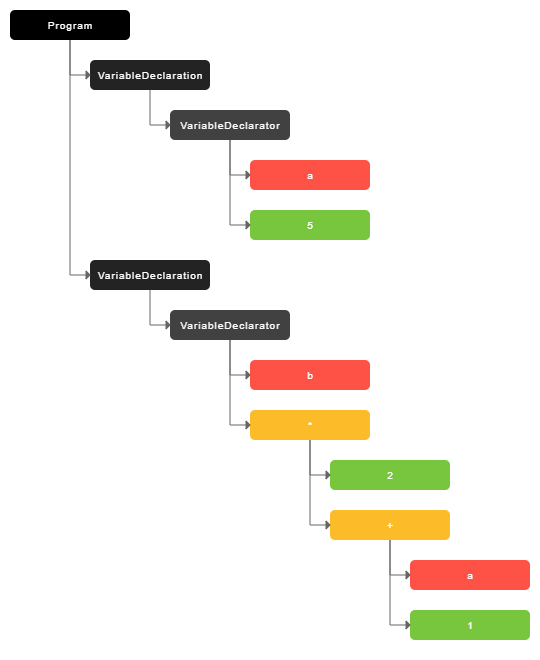
\includegraphics[scale=0.6]{img/ast.png}
  \caption{Пример абстрактного синтаксического дерева}
  \label{ast}
\end{figure}

На рисунке \ref{ast} представлен пример абстрактного синтаксического дерева, построенного для 
следующего фрагмента кода на языка JavaScript:
%  Дерево было построено с использованием парсера,
% входящего в состав транспайлера Babel. 

\lstinputlisting[language=JavaScript, style=linesWithNumbers]{listings/ast-expression.js}

Дерево было построено с использованием парсера, входящего в состав транспайлера Babel.

\subsubsection{Этапы работы Babel}

После того, как было получено представление о понятии AST, можно перейти к обзору основных этапов 
работы Babel, которые представлены на рисунке \ref{babel_stages}.
\begin{figure}[h!]
  \centering
  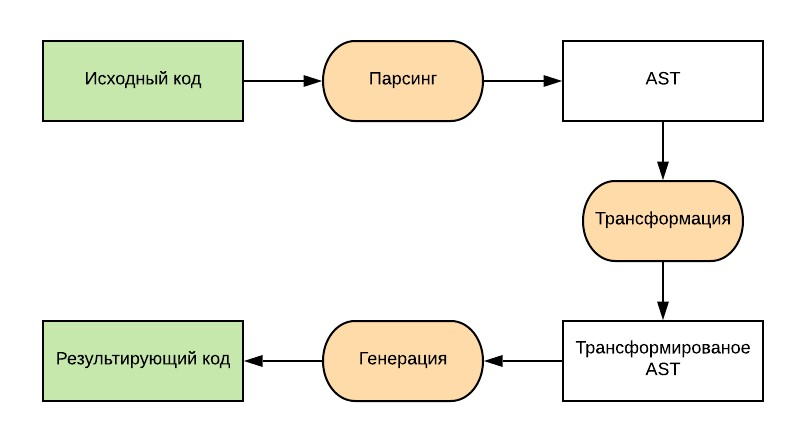
\includegraphics[scale=1.2]{img/babel_stages.jpg}
  \caption{Этапы работы Babel}
  \label{babel_stages}
\end{figure}

\subsubsection*{Парсинг}
На этом этапе код, передаваемый в Babel, конвертируется в абстрактное синтаксическое дерево. 
В свою очередь этап парсинга подразделяется на 
две фазы: \textit{лексический анализ} и \textit{синтаксический анализ}.

В ходе лексического анализа текст исходного кода преобразуется в массив токенов. По этой причине фазу 
лексического анализа часто называют токенизацией. Здесь токен - это объект, описывающий любую значащую 
подпоследовательность символов исходного кода. Например, фрагмент кода

\lstinputlisting[language=JavaScript, style=linesWithNumbers]{listings/fragment-for-tokenization.js}
будет преобразован в следующий массив токенов:

\lstinputlisting[language=JavaScript, style=linesWithNumbers]{listings/tokens.js}
Свойства start и end описывают положение токена в строке, loc $-$ строку, в которой был найден токен. 
Поле type указывает на объект, который хранит набор свойств, описывающих каждый отдельный токен:
\lstinputlisting[language=JavaScript, style=linesWithNumbers]{listings/token-type.js}

Далее следует так называемый синтаксический анализ, цель которого $-$ построение абстрактного 
синтаксического дерева на основе массива токенов, полученного на предыдущем этапе. В ходе этого 
процесса токены преобразуются в узлы дерева (Node), которые кроме уже описанных данных содержат также
информацию о типе узла. Примерами таких типов являются FunctionDeclaration, VariableDeclaration или 
ReturnStatement. Для рассмотренного выше фрагмента кода построенное парсером абстрактное синтаксическое 
дерево будет выглядеть следующим образом:

\lstinputlisting[language=JavaScript, style=linesWithNumbers]{listings/ast-for-fragment.js}

\subsubsection*{Трансформация}
Как только абстрактное синтаксическое дерево построено, начинается этап трансформации. На этом этапе 
производится рекурсивный обход, во время которого добавляются, заменяются или удаляются узлы дерева.
Трансформации, проводимые над деревом, определяются списком подключенных плагинов и применяются в 
порядке их следования в этом списке.

*Используется Посетитель, подробности далее* 

\subsubsection*{Генерация}
По окончании модификации, абстрактное синтаксическое дерево конвертируется обратно в код. 
Происходит это следующим образом: производится обход дерева в глубину, в процессе которого строится строка,
представляющая модифицированный код.

\subsubsection{Шаблон Посетитель}

Обход абстрактного синтаксического дерева, производимый на этапе трансформации, реализован с применением 
шаблона проектирования Посетитель. Это поведенческий шаблон проектирования, впервые описанный в книге 
``Приёмы объектно-ориентированного проектирования. Паттерны проектирования'' \cite{gang_of_4}.
Суть шаблона заключается в предоставлении возможности определять новые операции над объектами,
 не внося изменения в классы этих объектов.

% \subsubsection*{Решаемая проблема}
Проблема, которую решает шаблон Посетитель, можно сформулировать следующим образом:

Необходимо определить ряд несвязанных между собой операций над объектами, принадлежащими определенной структуре.
При этом, требуется избежать модифицирования кода классов этих объектов при добавлении новых операций. 

Шаблон Посетитель описывает решение этой проблемы так:
вместо того чтобы добавлять новое поведение в каждый объект структуры, необходимо вынести это поведение 
в отдельный класс посетителя. Таким образом объекты не будут выполнять операции самостоятельно, а вместо этого 
они будут передаваться в методы посетителя.

Посетитель, в свою очередь, будет содержать множество методов, обрабатывающих объекты разных типов, так как
поведение для них скорее всего будет отличаться. Вопрос, какой именно метод вызывать для каждого конкретного объекта,
разрешается с помощью механизма двойной диспетчеризации. Ответственность за вызов правильного метода посетителя
возлагается на сам объект, передаваемый посетителю в качестве аргумента. Для этого в каждом классе структуры
определяется специальный метод \code{accept(Visitor v)}, внутри которого происходит вызов метода посетителя, соответствующего
типу данного объекта.

На рисунке \ref{visitor_uml} представлена UML диаграмма, иллюстрирующая классическую реализацию шаблона
Посетитель. Диаграмма состорит из следующих компонентов:
\begin{itemize}
  \item \textbf{Visitor} $-$ описывает общий интерфейс для всех посетителей. Содержит объявления 
    методов \code{visit} для каждого конкретного типа элементов. 
  \item \textbf{ConcreteVisitor} $-$ конкретный класс посетителя, реализует интерфейс, определенный в Visitor.
  \item \textbf{Element} $-$ интерфейс, содержащий объявление метода \code{accept}.
  \item \textbf{ElementA / ElementB} $-$ конкретные классы элементов структуры, реализуют метод \code{accept}
    интерфейса Element, вызывая внутри него метод Посетителя, соответствующий своему типу.
  \item \textbf{Client} $-$ класс-пользователь структуры объектов. В нем происходит вызов метода \code{accept}
    объекта с конкретным экземпляром Посетителя.
\end{itemize}

\begin{figure}[h!]
  \centering
  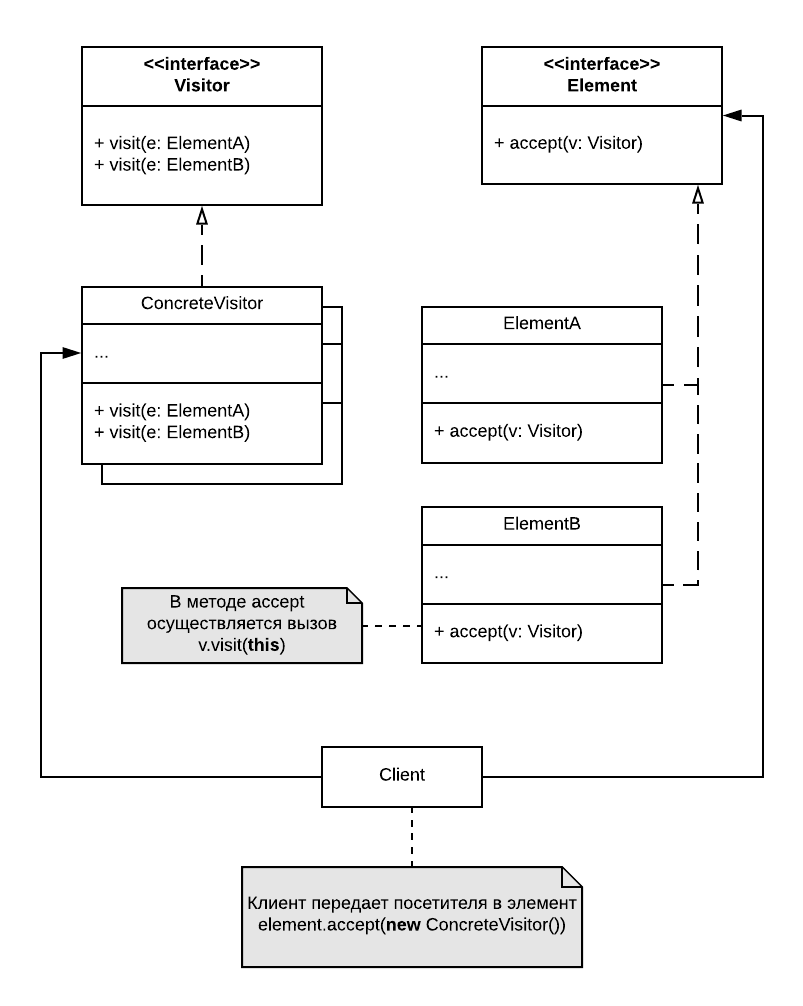
\includegraphics[scale=1.0]{img/visitor_uml.png}
  \caption{UML диаграмма компонентов шаблона Посетитель}
  \label{visitor_uml}
\end{figure}

Шаблон Посетитель широко используется в реализация различных компиляторов для определения операций над 
абстрактными синтаксическими деревьями. Babel, компилирующий JavaScript код в другой JavaScript код,
также не является исключением. Однако, из-за ограничений языка программирования JavaScript, таких как
отсутствие поддержки перегрузки методов и возможности определять интерфейсы, реализация шаблона Посетитель
в Babel несколько отличается от классической.

В Babel посетить представляет из себя обычный JavaScript объект, который содержит методы, чьи названия 
совпадают с типом узлов AST, которые они ``посещяют''.

\lstinputlisting[language=JavaScript, style=linesWithNumbers]{listings/visitor_expample.js}

Внутри методов Посетителя определяются операции, которые необходимо произвести над узлами данного типа.
Узлы абстрактного синтаксического дерева в Babel не содержат метода \code{accept}. Вместо этого за вызов
подходящего метода Посетителя отвечает функция \code{traverse}, выполняющая обход дерева. Ниже приведен 
псевдокод, упрощенно иллюстрирующий механизм работы этой функции.

\lstinputlisting[language=JavaScript, style=linesWithNumbers]{listings/traverse.js}

 *Плагины Babel - это по сути визиторы*

\pagebreak

\section{Babel API}

\pagebreak

\section{Создание синтаксической конструкции deep spread operator с помощью Babel}
% В данной главе описан процесс создания плагина для транспайлера Babel. В качестве 
\subsection{Постановка задачи}
Необходимо разработать плагин для транспайлера Babel, позволяющий использовать синтаксическую конструкцию
\code{deep spread} оператор в рамках JavaScript кода. 

Идея создания нового \code{deep spread} оператора навеяна существующим в языке JavaScript обычным \code{spread}
оператором, по этой причине для лучшего понимания вопроса следует сперва ознакомиться с ним.

\subsubsection{Обычный spread оператор}
Spread оператор (или оператор расширения)\cite{spread_mozilla} позволяет расширить итерируемые объекты и положить их 
содержимое в индивидуальные элементы. Оператор имеет синтаксис \code{...arg}, где 
\code{arg} может быть представлен объектом, массивом или строкой. Спецификация языка допускает следующие 
варианты использования этого оператора:
\begin{itemize}
  \item {Для функций. Позволяет отобразить элементы массива на аргументы функции при ее вызове.}
  \lstinputlisting[language=JavaScript, style=linesWithNumbers]{listings/spread-expample-func.js}
  \item {Для литералов массивов и строк. Позволяет использовать элементы массивов в качестве отдельных значений.}
  \lstinputlisting[language=JavaScript, style=linesWithNumbers]{listings/spread-example-array.js}
  \item {Для литералов объектов. Позволяет использовать пары ключ-значение исходного объекта в качестве отдельных значений.}
  \lstinputlisting[language=JavaScript, style=linesWithNumbers]{listings/spread-example-obj.js}
\end{itemize}
Важно отметить, что при использовании \code{spread} оператора создается копия элементов 
итерируемого объекта, к которому применяется оператор. По этой причине наиболее частым вариантом 
использования данного оператора является копирование массивов или объектов. В следующем фрагменте 
кода приведен пример создания копии объекта с использованием \code{spread} оператора:
\lstinputlisting[language=JavaScript, style=linesWithNumbers]{listings/copy-obj-with-spread.js}
Однако стоит обратить внимание на тот факт, что при копировании с использованием \code{spread} оператора
создается лишь неглубокая копия исходного объекта. Это означает, что при наличии вложенных структур, 
они будут скопированы по ссылке. 

\subsubsection{Deep spread оператор}
Deep spread оператор (или глубокий оператор расширения) $-$ это не существующий в стандарте языка ECMAScript оператор, поддержку которого 
планируется осуществить средствами транспайлера Babel в рамках данной выпускной квалификационной работы.

По задумке \code{deep spread} оператор должен повторять возможности обычного \code{spread} оператора с тем отличием,
что будет всегда создавать глубокие (рекурсивные) копии операндов. Новый оператор будет иметь синтаксис \code{...@arg},
где \code{arg} может быть представлен объектом или массивом. Ниже приведен пример потенциального 
использования подобного оператора.
\lstinputlisting[language=JavaScript, style=linesWithNumbers]{listings/copy-with-deep-spread.js}

\subsection{План работ}
Для того чтобы добавить поддержку новой синтаксической конструкции \code{deep spread} оператор в 
транспайлер Babel, потребуется выполнить следующую последовательность шагов:
\begin{enumerate}
  % \item ``Научить'' токенизатор Babel распознавать последовательность символов ``\code{...@}'' как самостоятельный токен.
  % \item Модифицировать парсер Babel таким образом, чтобы при построении абстрактного синтаксического дерева
  \item Расширить парсер Babel, добавив в него возможность распознавать последовательность символов 
    ``\code{...@}'' как обычный \code{spread} оператор, но с флагом \code{deep = true}.  
  % \item Расширить парсер Babel (добавить возможность распознавать новый вид токена и модифицировать узел AST типа spread expression, добавив флаг deep )
  \item Написать плагин для Babel, позволяющий оборачивать операнд \code{deep spread} оператора в вызов функции рекурсивного копирования.
  % \item Протестировать полученные результаты
\end{enumerate}

\subsection{Используемые инструменты}
git, make, github, vscode, nodejs, yarn, babel v7

*Описать подробно*
\subsection{Ход работы}
Согласно составленному плану работ первым делом необходимо расширить возможности транспайлера Babel таким образом,
чтобы он смог корректно распознавать новый синтаксис. Для этого следует сделать форк репозитория Babel,
расположенного на сервисе GitHub по адресу \url{https://github.com/babel/babel}. Создание форка - это
получение собственной копии чужого проекта с целью внести изменения или исправления ошибок. При желании
из скопированного с помощью форка репозитория можно сделать Pull Request в оригинальный репозиторий,
таким образом предложив внести свои изменения в основной проект.
\begin{figure}[h!]
  \centering
  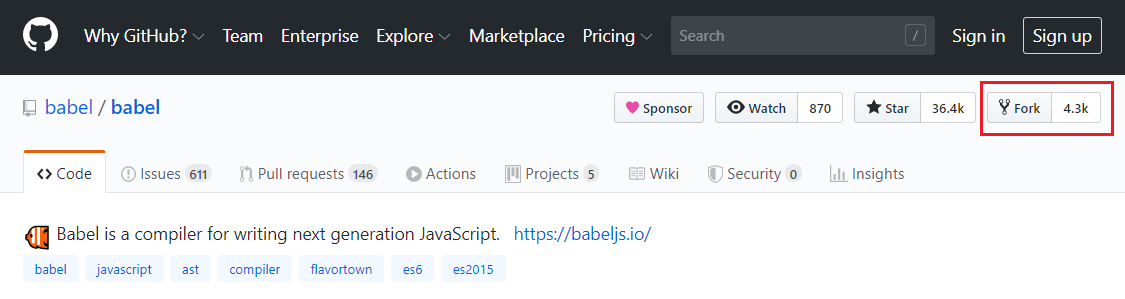
\includegraphics[scale=0.55]{img/babel_fork.PNG}
  \caption{Создание форка проекта Babel}
  \label{babel_fork}
\end{figure}

После того как сделан форк проекта, следует получить локальную копию репозитория проекта, выполнив следующую команду:
\begin{lstlisting}
 > git clone https://github.com/{github_name}/babel.git
\end{lstlisting}

Проект Babel организован в виде монорепозитория. Это означает, что код множества независимых подпроектов,
таких как babel-parser или babel-cli, хранится в одном git репозитории. Структура репозитория Babel
представлена на рисунке \ref{babel_dirs}.

\begin{figure}
\centering
\framebox[\textwidth]{%
\begin{minipage}{0.9\textwidth}
  \dirtree{%
    .1 babel.
    .2 packages.
    .3 babel-cli.
    .3 babel-parser.
    .3 babel-plugin-transform-classes.
    .3 babel-traverse.
    .3 \ldots .
    .2 Gulpfile.js.
    .2 Makefile.
    .2 \ldots.
  }
\end{minipage}
}
\caption{Структура репозитория Babel}
\label{babel_dirs}
\end{figure}


Независимые пакеты, входящие в состав Babel, находятся в директории \code{packages/}. Для того, чтобы 
расширить парсер, необходимо внести изменения в пакет babel-parser.

Первым делом следует ``научить'' токенизатор Babel распознавать последовательность символов ``\code{...@}'' 
как самостоятельный токен. Все поддерживаемые при парсинге токены перечислены в экспортируемом объекте 
\code{types} в файле \code{babel/packages/babel-parser/src/tokenizer/types.js}. Чтобы включить поддержку нового токена,
следует добавить новое поле в объект \code{types}. Название поля должно соответствовать имени токена, а
в качестве значения следует передать результат вызова функции-конструктора нового токена с оператором \code{new}. 

\lstinputlisting[language=JavaScript, style=linesWithNumbers, caption={Объект types, содержащий поддерживаемые типы токенов}]{listings/add-new-token.js}

Далее требуется внести изменения в сам токенизатор Babel таким образом, чтобы при появлении последовательностей символов 
``\code{...@}'' в тексте исходного кода создавался объявленный ранее токен \code{ellipsisAt}. Для этого 
перейдем в файл \code{babel/packages/babel-parser/src/tokenizer/index.js} и
добавим дополнительное условие в метод \code{readToken\_dot()} класса \code{Tokenizer}, ответственный за распознавание токенов,
содержащих символ ``.'' (точка).
\lstinputlisting[language=JavaScript, style=linesWithNumbers, label={readTokenDot}, caption=Метод readToken\_dot() класса Tokenizer]{listings/add-condition-to-tokenizer.js}

На листинге \ref{readTokenDot} выделены строки кода, добавленные для того чтобы токенизатор Babel 
получил способность корректно распознавать описанную выше последовательность символов. В них происходит 
проверка на факт наличия символа ``@'' (в английском именуемого как ``at'') за тремя подряд идущими  
символами ``.'' (точка). Если такой символ найден, то создается токен \code{ellipsisAt}, в противном случае
$-$ простой \code{ellispis} (с английского $-$ многоточие).

После того как в токенизатор Babel была добавлена возможность распознавать токен \code{ellipsisAt},
следует также внести изменения в сам парсер. Чтобы понять, какие именно требуются изменения, посмотрим на то, какое
синтаксическое дерево строится для выражения, содержащего обычный \code{spread} оператор. Для этого будем использовать 
инструмент AST Explorer (\url{https://astexplorer.net}), в котором выберем язык JavaScript и парсер babel-v7.
Введем строку кода \code{const a = \{...\{c: 1\}\}} в панель слева и наведем курсор на интересующий 
нас \code{spread} оператор. Узел абстрактного синтаксического дерева, соответствующий выделенному оператору,
отобразится на панели справа. Как видно на рисунке \ref{ast_explorer}, в данному случае узел имеет тип 
\code{SpreadElement}.

\begin{figure}[h!]
  \centering
  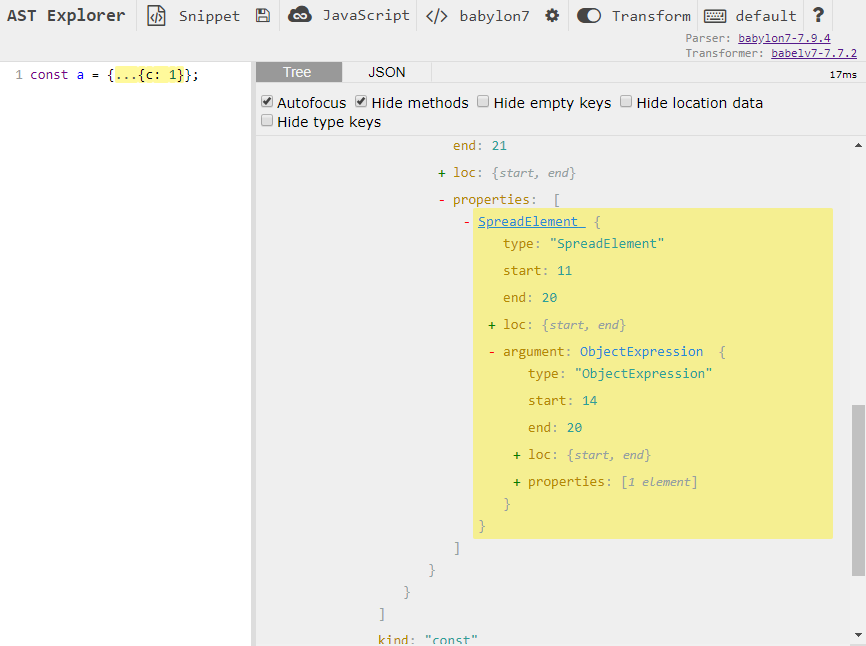
\includegraphics[scale=0.7]{img/ast-explorer.png}
  \caption{Исследование синтаксического дерева выражения с помощью AST Explorer}
  \label{ast_explorer}
\end{figure}


Добавим новый атрибут \code{deep: boolean} в тип узла \code{SpreadElement}. Новый атрибут будет указывать,
должен ли \code{spread} оператор возвращать рекурсивную копию операнда $-$ в случае с \code{deep spread} оператором,
или нет $-$ в случае с обычным \code{spread} оператором. Так как все типы узлов синтаксического дерева 
определены в файле \code{babel/packages/babel-parser/src/types.js}, именно в него и нужно внести изменения. 

\lstinputlisting[language=JavaScript, style=linesWithNumbers, label={addDeepAttr}, caption={Добавление атрибута deep в тип узла SpreadElement}]{listings/add-deep-attr.js}
% Первым делом добавим новый атрибут \code{deep: boolean}
% в тип \code{SpreadElement}, описывающий соответствующий узел абстрактного синтаксического дерева (листинг \ref{addDeepAttr}).
% Все типы узлов дерева определены в файле \code{babel/packages/
% babel-parser/src/types.js}


% Посмотрим на обычный SpreadExpression через AST explorer 
Для того чтобы новый атрибут корректно инициализировался, требуется также изменить метод \code{parseSpread} класса
\code{LValParser}, объявленного в файле \code{babel/packages/babel-parser/src/parser/lval.js} (листинг \ref{parseSpread}). 
Добавим в метод новый аргумент \code{isDeep: boolean} со значением \code{false} по умолчанию. Значение этого аргумента будем записывать 
в поле \code{deep} создаваемого узла.

\lstinputlisting[language=JavaScript, style=linesWithNumbers, label={parseSpread}, caption={Добавление аргумента isDeep в метод parseSpread класса LValParser}]{listings/parse-spread.js}

\subsection{Результат}
\pagebreak
\section{Заключение}
\pagebreak

\addcontentsline{toc}{section}{Список литературы}
\begin{thebibliography}{9}
  \bibitem{ecma-262} Стандарт ECMA-262 [Электронный ресурс] $-$ Режим доступа: \linebreak
    \url{https://www.ecma-international.org/publications/standards/Ecma-262.htm}
  \bibitem{documentation} Документация Babel [Электронный ресурс] $-$ Режим доступа: \linebreak
    \url{https://babeljs.io/docs/en}
  \bibitem{traceur} Документация Traceur [Электронный ресурс] $-$ Режим доступа: \linebreak
    \url{https://github.com/google/traceur-compiler/wiki/Getting-Started}
  \bibitem{jstransform} Репозиторий JSTransform на сервисе GitHub [Электронный ресурс] $-$ Режим доступа:
    \url{https://github.com/facebookarchive/jstransform}
  \bibitem{gang_of_4} Э. Гамма, Р. Хелм, Р. Джонсон, Д. Влиссидес. Приёмы объектно-ориентированного проектирования. Паттерны проектирования, СПб.: Питер, 2017. $-$ 368 с.: ил.
  \bibitem{spread_mozilla} Описание spread синтаксиса на ресурсе MDN web docs [Электронный ресурс] $-$ Режим доступа:
    \url{https://developer.mozilla.org/en-US/docs/Web/JavaScript/Reference/Operators/Spread_syntax}
\end{thebibliography}
\end{document}